% Template for FPL 2012 papers; to be used with:
%          spconf.sty   - ICASSP/ICIP LaTeX style file
%          IEEEtran.bst - IEEE bibliography style file

% Created:  Apr-May 2005 - Riku Uusikartano -- riku.uusikartano@tut.fi
% Modified: March-2012 - Daniel Mu�oz Arboleda -- damuz@unb.br
% --------------------------------------------------------------------------

\documentclass[10pt,a4paper]{article}

\usepackage{spconf,amsmath,epsfig}
\usepackage[brazilian]{babel} % Suporte para o Portugu�s
\usepackage[latin1]{inputenc} % Suporte para acentua��o sem necessidade dos comandos especiais.
\usepackage[]{subfigure}
\usepackage[portuguese,algoruled,longend]{algorithm2e}
\usepackage{multirow}



% Titulo do documento
% -------------------
\title{Ponto de controle 1a \\ Controle de acesso com  face humana}


% Nome dos autores
% ----------------
\name{
Ant�nio Ald�sio - 14/0130811 ---- Vitor Carvalho de Almeida - 14/0165380}
\address{Programa de Gradua��o em Engenharia Eletr�nica, Faculdade Gama\\
Universidade de Bras�lia\\
Gama, DF, Brasil\\\\
email: aldisiofilho@gmail.com ---- vitorcarvalhoamd@gmail.com }


\hyphenation{Tam-pe-re ela-bo-ra-cao}

\begin{document}

\maketitle

\begin{resumo}



\textbf{Palavras-chave:} Controle de acesso,raspberry pi,opencv.

\end{resumo}
\section{Introdu��o}


\section{Desenvolvimento}


\subsection{Descri��o do Hardware}

Foi montado um sistema de ativa��o da trava eletr�nica. Utilizando os seguintes materiais:

\begin{itemize}
\item Trava solenoide 12V (figura \ref{trava});
\item Fonte DC 12V ;
\item Resistor de 1 KOhm;
\item Transistor NPN (TIP41);
\item Jumpers
\item Protoboard
\end{itemize}


\begin{figure}[h!]
\caption{Trava eletr�nica solenoide 12V}
\centering % para centralizarmos a figura
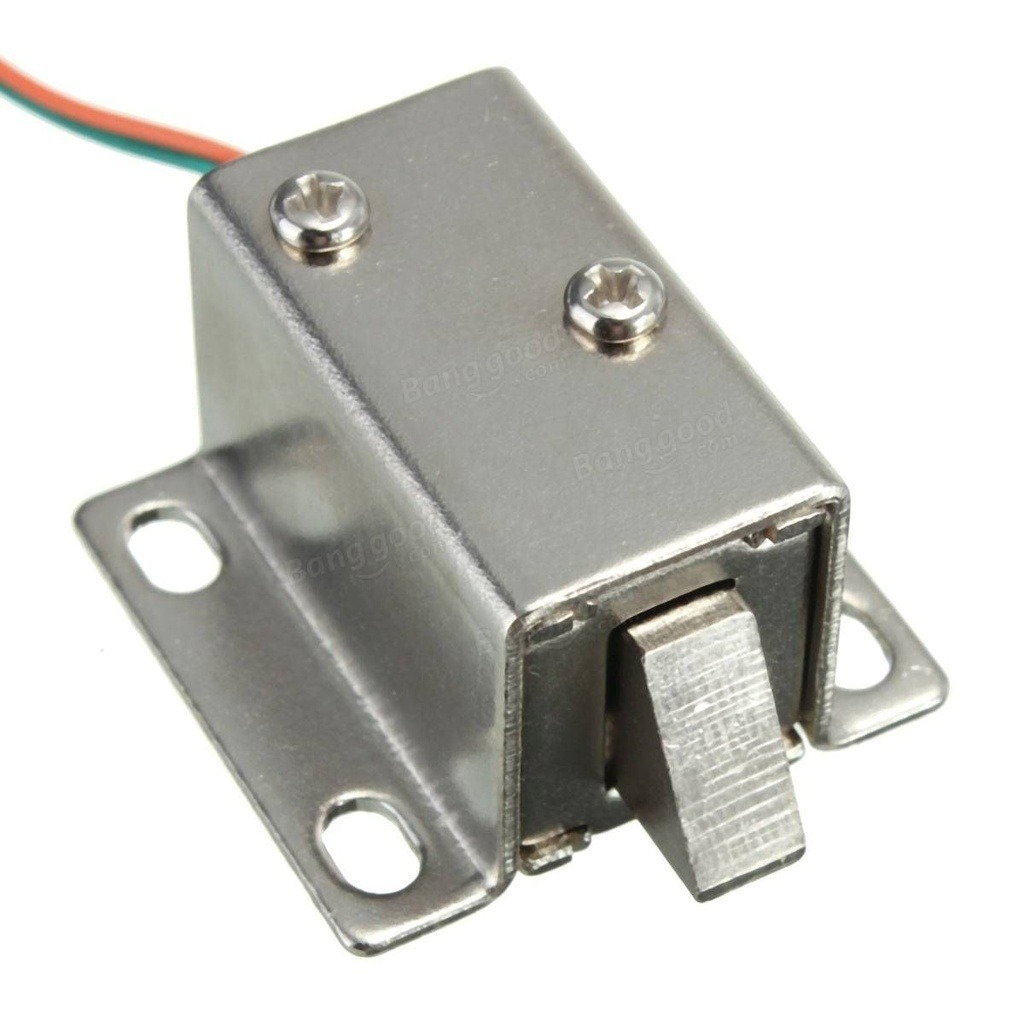
\includegraphics[width=5cm]{trava.jpg} % leia abaixo
\label{trava}
\end{figure}

Na protoboard foi montado o circuito da figura \ref{circuito}.

\begin{figure}[h!]
\caption{Ativa��o da trava eletr�nica solenoide 12V}
\centering % para centralizarmos a figura
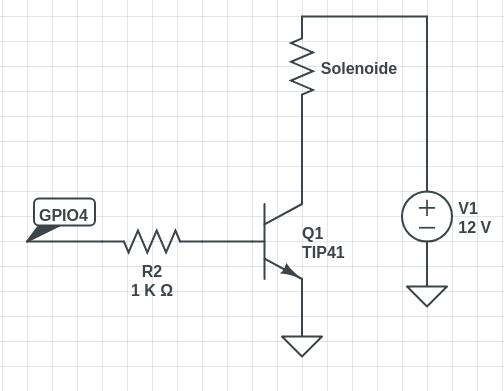
\includegraphics[width=5cm]{circuito_trava.jpg} % leia abaixo
\label{circuito}
\end{figure}

O pino de entrada foi conectado � GPIO4 da Raspberry Pi 3 para que fossem enviados os comandos para abrir a porta. 

A trava solenoide mantem a porta fechada at� que seja inserida uma tens�o de 12V em seus terminais. Neste momento, o solenoide faz com que o ''dente'' da trava seja retra�do, liberando a abertura da porta. Ao retirar a tens�o dos terminais, uma mola retorna a trava para a posi��o original, travando a porta novamente. [2]

Foi utilizada uma fonte DC de 12V - 2A com conex�o Jack P4, ligada na protoboard com um conector Jack P4 f�mea.

Foi conectada uma caixa de som � sa�da P2 da Raspberry Pi para reproduzir sons de confirma��o ou nega��o de acesso.


Para receber a requisi��o de acesso, foi montado um circuito com bot�o em modo Pull-Up, como mostra o esquematico da figura \ref{botao}

\begin{figure}[h!]
\caption{Bot�o em modo Pull-Up}
\centering % para centralizarmos a figura
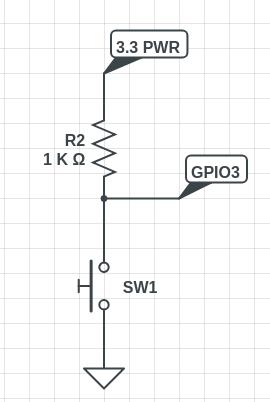
\includegraphics[width=5cm]{circuito_botao.jpg} % leia abaixo
\label{botao}
\end{figure}


\subsection{Descri��o do Software}

\subsubsection{Campainha}

A GPIO3 foi configurada de modo a ficar em modo 

\lstset{language=bash,
	numbers=left,
	linewidth=8cm,
	breaklines}
\begin{lstlisting}
Modo de espera
Bot�o foi pressionado? N-Espera S-Segue
Envia requisi��o de acesso para o c�digo principal.
\end{lstlisting}



\subsubsection{Resposta ao usu�rio}

A rotina para liberar a porta foi feita em um arquivo de instru��es bash. O c�digo \textit{abre.sh} � mostrado no apendice.

\begin{itemize}

\item[1]Primeiramente � reproduzido o som de uma confirma��o de acesso pela caixa de som, para que o usu�rio saiba que pode entrar

\item[2] Depois a GPIO4 � definida como sa�da e colocada em n�vel l�gico alto.


\item[3] � definido um tempo de espera, no caso 3 segundos, para que a trava se mantenha retra�da e o usu�rio possa empurrar a porta.

\item[4] Ao final da contagem a GPIO4 volta para o n�vel l�gico baixo. Neste momento, ao encostar a porta, esta ser� trancada.

\item[5] Por fim, a GPIO4 � liberada para uso em outra rotina.

\end{itemize}





Caso o usu�rio n�o tenha acesso cadastrado, ao tocar a campainha deve ser executado o c�digo \textit{negado.sh}, mostrado abaixo

\lstset{language=bash,
	numbers=left,
	linewidth=8cm,
	breaklines}
\begin{lstlisting}
#!/bin/bash

omxplayer -o local /home/pi/embarcados/projeto_final/sons/nao.mp3
\end{lstlisting}

Neste caso, a �nica fun��o realizada � a reprod��o de um som de nega��o na caixa de som.
%\section{Resultados}

[FOTO CIRCUITO]


A ativação da trava eletrônica foi realizada com sucesso, sem sobreaquecimento do transistor, nem falha na comunicação.

%\section{Discuss�o e Conclus�es}


Pelos experimentos realizados, concluiu-se que o projeto pode ser implementado da forma como foi pensado inicialmente, pois a comunica��o da Raspberry Pi com os perif�ricos (trava, bot�o, c�mera) funcionou corretamente.

Com o sistema rodando no computador so vimos um pequeno atraso da imagem com a indentifica��o, isso n�o ser� um problema para nosso projeto, pois iremos realizar uma foto. O que pode ser um problema � o delay do reconhecimento com a abertura da porta.

A bibliotecas de reconhecimento facial OpenCV e face$\_$recognition funcionaram corretamente no notebook, ainda falta implement�-las na Raspberry Pi.

Uma limita��o das bibliotecas � que elas n�o diferenciam rostos reais de rostos em fotos mostradas para a c�mera. Isso � um grande problema de seguran�a para o projeto, por�m a dupla j� est� estudando t�cnicas de diferencia��o destes casos.

Decidiu-se usar o bot do Telegram como interface do administrador com o sistema, porque assim o acesso � muito mais pr�tico e podem ser recebidas notifica��es no celular sem necessidade de instala��o de outros aplicativos.

Em rela��o ao servidor e cliente � uma boa escolha a utiliza��o da API do telegram, pois assim tornamos o acesso ao sistema remotamente super f�cil e acessivel a qualquer usu�rio que tenha o minino de conhecimento em mensageiros de comunica��o. Por outro lado a sua programa��o ser� um pouco trabalhosa , pois ser� necess�rio considerar as varia��es de entrada do usu�rio para uma mesma a��o.

Para este documento, foram escritos programas cuja rotina principal � espec�fica para cada a��o. Por�m, para o pr�ximo ponto de controle, os c�digos ser�o unidos como subrotinas de um c�digo principal de controle do sistema.


\small
% IEEEtran is a LaTeX style file defining the reference formatting.
% -----------------------------------------------------------------
\section{Referencias}

 \begin{description}
 

 \item[[ 1]] https://github.com/opencv/opencv
 \item[[ 2]] https://www.filipeflop.com/blog/acionando-trava-eletrica-com-rfid/
  \end{description}



\end{document}